% -*- TeX-engine: xetex; TeX-PDF-mode: t; -*-
\def\pgfsysdriver{pgfsys-dvipdfmx.def}
%% ---------------------------------------------------------------------------- %
% Beamer basics
% The beamer class automatically loads some other \LaTeX packages, including
% xcolor, amsmath, amsthm, calc, geometry, hyperref, extsizes.
% color predefined:red, blue, green, cyan, magenta, yellow, black, darkgray, gray,
% lightgray, orange, violet, purple, brown

% \documentclass[pdf]{beamer}
% aspectratio=1610
% default font size 11pt;8pt, 9pt, 10pt, 11pt, 12pt, 14pt, 17pt, 20pt
\documentclass[11pt]{beamer}

\mode<article> % 仅应用于article版本
{
  \usepackage{beamerbasearticle}
  \usepackage[xetex]{hyperref}
}

%% ---------------------------------------------------------------------------- %
% themes

% http://www.hartwork.org/beamer-theme-matrix/
% Antibes, Bergen, Berkeley, Berlin, Boadilla, Copenhagen, Darmstadt, Dresden,
% Frankfurt, Goettingen, Hannover, Ilmenau, Juanlespins, Madrid, Malmoe,
% Marburg, Montpellier, Paloalto, Pittsburgh, Rochester, Singapore, Warsaw
\usetheme[compress]{Singapore} %title at the top-middle
% \usetheme{Manhattan}
% \usetheme{Boadilla}
\usetheme{keynote-gradient}
% \usetheme{lankton-keynote}
\beamertemplatetransparentcoveredhigh
% \beamertemplatetransparentcovereddynamicmedium

% font themes
% \usefonttheme[onlymath]{serif}
% \usefonttheme{structureitalicserif}
% \usefonttheme{structurebold}
% \usefonttheme{structuresmallcapsserif}
% \usepackage{lucidaso} % Lucida Bright (SO Version)
\usefonttheme[onlymath]{serif}
% \usepackage[small]{eulervm} % Euler VM for math font
% \usepackage{helvet}

% color themes:albatross crane beetle dove fly seagull wolverine beaver
% \usecolortheme{fly}
% Outer color themes:whale, seahorse, dolphin
\usecolortheme{whale}
% Inner color themes: lily, orchid,rose
\usecolortheme{orchid}

% rectangles circles inmargin rounded
\useinnertheme{rectangles}
% \useinnertheme[shadow]{rounded}
% infolines miniframes shadow sidebar c smoothtree split tree progressbar
% \setbeamertemplate{navigation symbols}{} % no navigation
% \useoutertheme{progressbar}

% define colors
% \setbeamercolor{uppercol}{fg=white,bg=blue}%
\setbeamercolor{lowercol}{fg=black,bg=gray}%
\xdefinecolor{lavendar}{rgb}{0.8,0.6,1}
\xdefinecolor{olive}{cmyk}{0.64,0,0.95,0.4}
\xdefinecolor{mygreen}{rgb}{0,0.6,0}
\xdefinecolor{mygray}{rgb}{0.5,0.5,0.5}
\xdefinecolor{mymauve}{rgb}{0.58,0,0.82}
\xdefinecolor{mycolor}{rgb}{0.08,0.08,0.16}

% redefine structure color
% \usecolortheme[named=yellow]{structure}
% redefine alert color
% \setbeamercolor{alerted text}{fg=cyan}
\setbeamercolor{block title alerted}{fg=white,bg=violet!40!gray}
\setbeamercolor{block body alerted}{fg=black!90,bg=white}
% \setbeamercolor{alerted text}{fg=green}

% \colorlet{structure}{green!60!black}
\colorlet{alert}{green!60!black}

\setbeamertemplate{headline}[default]

% \beamertemplateshadingbackground{blue!5}{yellow!10}
% \setbeamertemplate{background canvas}[vertical
% shading][top=blue!30,bottom=white,middle=blue!20,midpoint=.4]
% \setbeamertemplate{sidebar canvas
% left}[horizontal shading][left=white!40!black,right=black]
% \mode<beamer>{\setbeamertemplate{blocks}[rounded][shadow=true]}
% transparent,highly dynamic,dynamic,
\setbeamercovered{invisible}
\setbeamercolor{body}{fg=blue!80, bg=black!20}
\setbeamercolor{head}{fg=blue,bg=blue!30}

\setbeamerfont{title}{shape=\slshape,family=\ttfamily,series=\bfseries}

% \addtobeamertemplate{block begin}{%
%   \setlength{\textwidth}{0.9\textwidth}%
% }{}

\beamertemplateballitem

%% ---------------------------------------------------------------------------- %
% useful packages

% math (symbols) related
\usepackage{pifont}
\usepackage{mathrsfs}
\usepackage{bbding}
\usepackage{amsmath, amsfonts, amssymb}
% \usepackage{textcomp}
\usepackage{indentfirst}

% \usepackage{pgf,pgfarrows,pgfnodes,pgfautomata,pgfheaps}
% \usepackage{subfigure}
\usepackage{times}
\usepackage{tikz}
\usepackage[tikz]{bclogo}
\usepackage{graphicx}
\usepackage{graphviz}
\usepackage{ccaption}
\graphicspath{{figure/}{fig/}{logo/}{logos/}{graph/}{graphs}}
\DeclareGraphicsExtensions{.pdf,.eps,.png,.jpg,.jpeg}

\usepackage{fancybox} % shadowbox,fbox,Ovalbox,ovalbox,doublebox
\usepackage{multimedia}
\usepackage{listings}
\usepackage{boxedminipage}
\usepackage{multirow, multicol, pdflscape}
\usepackage{array}
\usepackage{ulem,soul}
% \usepackage{enumitem}
\usepackage[lined,boxed,ruled,linesnumbered]{algorithm2e}

%% randomly add text
% \usepackage{lipsum}
% \usepackage{blindtext}
%% ---------------------------------------------------------------------------- %
% definitions


\makeatletter
\newenvironment{CenteredBox}{%
  \begin{Sbox}}{%
  \end{Sbox}\centerline{\parbox{\wd\@Sbox}{\TheSbox}}}
\makeatother

\newenvironment<>{varblock}[2][\textwidth]{%
  \setlength{\textwidth}{#1}
  \begin{actionenv}#3%
    \def\insertblocktitle{#2}%
    \par%
    \usebeamertemplate{block begin}}
  {\par%
    \usebeamertemplate{block end}%
  \end{actionenv}}

%% ---------------------------------------------------------------------------- %
% settings

\makeatletter
\def\beamer@linkspace#1{%
  \begin{pgfpicture}{0pt}{-1.5pt}{#1}{5.5pt}
    \pgfsetfillopacity{0}
    \pgftext[x=0pt,y=-1.5pt]{.}
    \pgftext[x=#1,y=5.5pt]{.}
  \end{pgfpicture}}
\makeatother

\AtBeginSection[]{
  \frame<handout:0>{
    \frametitle{目录}
    \tableofcontents[current,currentsubsection]
  }
  \addtocounter{framenumber}{-1}%
}

\hypersetup{pdfpagemode={FullScreen}}
\hypersetup{pdfstartview={FitH}}
\setbeamertemplate{itemize/enumerate body begin}{\small}
\setbeamertemplate{itemize/enumerate subbody begin}{\footnotesize}
\lstset{ %
  backgroundcolor=\color{white},   % choose the background color
  basicstyle=\color{black}\ttfamily\tiny,        % the size of the fonts that are used for the code
  breakatwhitespace=false,         % sets if automatic breaks should only happen at whitespace
  breaklines=true,                 % sets automatic line breaking
  captionpos=b,                    % sets the caption-position to bottom
  commentstyle=\color{mygray}\itshape,    % comment style
  deletekeywords={...},            % if you want to delete keywords from the given language
  escapeinside={\%*}{*)},          % if you want to add LaTeX within your code
  extendedchars=true,              % lets you use non-ASCII characters; for 8-bits encodings only, does not work with UTF-8
  % frame=single,                    % adds a frame around the code
  keepspaces=true,                 % keeps spaces in text, useful for keeping indentation of code (possibly needs columns=flexible)
  keywordstyle=\color{blue!70},       % keyword style
  identifierstyle=\texttt,
  % language=C,                      % the language of the code
  morekeywords={*,...},            % if you want to add more keywords to the set
  numbers=left,                    % where to put the line-numbers; possible values are (none, left, right)
  numbersep=5pt,                   % how far the line-numbers are from the code
  numberstyle=\tiny\color{mygray}, % the style that is used for the line-numbers
  rulecolor=\color{black},         % if not set, the frame-color may be changed on line-breaks within not-black text (e.g. comments (green here))
  showspaces=false,                % show spaces everywhere adding particular underscores; it overrides 'showstringspaces'
  showstringspaces=false,          % underline spaces within strings only
  showtabs=false,                  % show tabs within strings adding particular underscores
  stepnumber=1,                    % the step between two line-numbers. If it's 1, each line will be numbered
  stringstyle=\color{mymauve},     % string literal style
  tabsize=2,                       % sets default tabsize to 2 spaces
  title=\lstname                   % show the filename of files included with \lstinputlisting; also try caption instead of title
}

\DeclareRobustCommand\nobreakspace{\leavevmode\nobreak\ }
\renewcommand{\baselinestretch}{1.3}
\renewcommand{\contentsname}{\setmainfont{KaiTi}目录\setmainfont{SimSun}}
\renewcommand{\figurename}{\setmainfont{Heiti}图\setmainfont{SimSun}}
\renewcommand{\tablename}{\setmainfont{Heiti}表\setmainfont{SimSun}}
\renewcommand{\refname}{\setmainfont{Heiti}参考文献\setmainfont{SimSun}}
% \renewcommand{\algorithmcfname}{算法}
\renewcommand{\today}{\number\year 年 \number\month 月 \number\day 日}

%% ---------------------------------------------------------------------------- %
% specific for this article
\newcommand{\dryrun}{\textmd{SERAPH}}
\newcommand{\rbscope}{\texttt{rbscope}}

\newcommand{\bug}{\ensuremath{\mathcal{B}}}
\newcommand{\patch}{\ensuremath{\mathcal{P}}}
\newcommand{\prog}{\ensuremath{\mathcal{S}}}
\newcommand{\bs}{\ensuremath{_{bug}}}
\newcommand{\ass}{\ensuremath{_{assert}}}
\newcommand{\entry}{\ensuremath{_{entry}}}
\newcommand{\ps}{\ensuremath{_{root}}}
\newcommand{\scope}{\ensuremath{_{scope}}}
%% ---------------------------------------------------------------------------- %
% font related
\usepackage[T1]{fontenc}
\usepackage[CJKchecksingle, CJKnumber]{xeCJK}  %specified for XeTeX, based on fontenc
\punctstyle{kaiming} % quanjiao, banjiao, hangmobanjiao, plain
% \usepackage[UTF-8, nofonts]{ctex}
\setmainfont[Mapping=tex-text]{TeX Gyre Termes}
\setsansfont[Mapping=tex-text]{TeX Gyre Termes}
\setmonofont[Mapping=tex-text]{Consolas}
\setbeamerfont{frametitle}{family=\rmfamily,series=\bfseries,size={\fontsize{10}{10}}}
% fontenc: BoldItalicFont, SlantedFont, BoldSlantedFont, SmallCapsFont
\setCJKmainfont[BoldFont={Adobe Heiti Std},ItalicFont={Adobe Kaiti Std}]{Adobe
  Song Std} %\bffamily, \itfamily
\setCJKmonofont{Adobe Heiti Std} %\ttfamily
\setCJKsansfont{Adobe Fangsong Std} %\sffamily

\newCJKfontfamily[youyuan]\youyuan{YouYuan}
\newCJKfontfamily[lishu]\lishu{LiSu}
\newCJKfontfamily[shuti]\shuti{FZShuTi}
\newCJKfontfamily[xinkai]\xinkai{STXingkai}

%% ---------------------------------------------------------------------------- %

\title{基于选择性符号执行的补丁验证}
\author{\\指导老师:\textit{赵建军}\\学\quad\quad 生:\textit{陈泓旭}}
% \date{\today}
\date{2014年1月7日}

\begin{document}

\frame{\titlepage}

\part{课题综述}
\frame{\partpage}

\begin{frame}
  \frametitle{研究背景}
  \transdissolve<1-5>
  \transblindshorizontal<6>
  \onslide<1->{程序演化过程中经常需要修复程序中的\textit{错误},不恰当的
  \textit{补丁程序}会造成极大的后果;\alert<6->{正确}并\alert<6->{高效}
  地进行补丁验证对提高软件质量及程序员生产效率至关重要。}\\
\vspace{2pt}

  \onslide<3->{\textit{常见的提高补丁程序质量的方法}:}
  \begin{enumerate}
  \onslide<4->{\item \textsf{静态分析}
    \begin{itemize}
    \item 检查是否满足特定的错误模式
    \item 分析可能出错的程序片段
    \end{itemize}}

  \onslide<5->{\item \textsf{软件测试}
    \begin{itemize}
    \item 手动测试
    \item 自动化测试 $\rightarrow$ 符号执行
    \end{itemize}}

  \end{enumerate}

\end{frame}

\begin{frame}[containsverbatim]
  \frametitle{一个典型的例子}
  \vspace{-5pt}
  % \begin{CenteredBox}
\begin{lstlisting}[language={[ANSI]C}]
 %* \color{mygray}{{case PSP\_COMP\_RLE: { }} *)
 %* \color{mygray}{{q = pixels[0] + offset;}} *)
 %* \color{mygray}{{endq = q + npixels * bytespp; }} *)
 %* \color{mygray}{{buf = g\_malloc (127); }} *)
  while (q < endq) {
    %* \color{mygray}{{p = buf; }} *)
    fread (&runcount, 1, 1, f);
    if (runcount > 128) {
      runcount -= 128;
      %* \color{mygray}{{fread ($\&$byte, 1, 1, f); }} *)
      %* \color{mygray}{{memset (buf, byte, runcount); }} *)
    }%* \color{mygray}{{ else  fread (buf, runcount, 1, f); }} *)
    %* \sout{\texttt{runcount = MIN(runcount, endq - q);}} *)
    %* \color{mygreen}{\texttt{runcount = MIN(runcount, (endq-q)/bytespp);}} *)
    if (bytespp == 1) {
      assert (q + runcount < endq);
      %* \color{mygray}{{memmove (q, buf, runcount); }} *)
      q += runcount;
    } else {
      %* \color{mygray}{\texttt{p = buf;}} *)
      for (i = 0; i < runcount; i++) {
        assert (q < endq);
        %* \color{mygray}{{*q = *p++; }} *)
        q += bytespp;
      }} }
  %* \color{mygray}{{g\_free (buf); break; }} *)
\end{lstlisting}
  % \end{CenteredBox}
\end{frame}

\begin{frame}
  \frametitle{本文的工作}
  \begin{enumerate}
  \item 提出了一种新的补丁验证的方法,使得可以通过\textit{有选择的符号执行}对补丁进行有效并高效地验证。
  \item 给出了从程序补丁处至错误发生处的\textit{极小相关程序片段}的算法。
  \item 给出了如何由现有程序的\rbscope 生成可供验证驱动程序进行\textit{交叉验证}的算法,使得可以通过符号执行结果对\textit{“补丁程序是否完整或引入新的错误”}这一问题给出正确解释。
  \item 实现了该思想的\textit{工具原型} \dryrun ,使得可以对 Coreutils 等实际复杂程序中的补丁进行验证。
  \end{enumerate}
\end{frame}


\part{ \dryrun 的实现}
\frame{\partpage}

\begin{frame}
  \frametitle{\dryrun 完整工作流程}
  \transdissolve<1-2>
  \only<1>{{\begin{alertblock}{\lishu{符号执行引擎的工作流}}
  \begin{figure}[t]
    \begin{center}
      
\includegraphics[width=.75\textwidth]{fig/se_workflow.pdf}\\
    \end{center}
  \end{figure}
  \end{alertblock}}}
\pause
  \only<2>{{\begin{alertblock}{\lishu{\dryrun 的工作流}}
  \begin{figure}[t]
    \begin{center}
      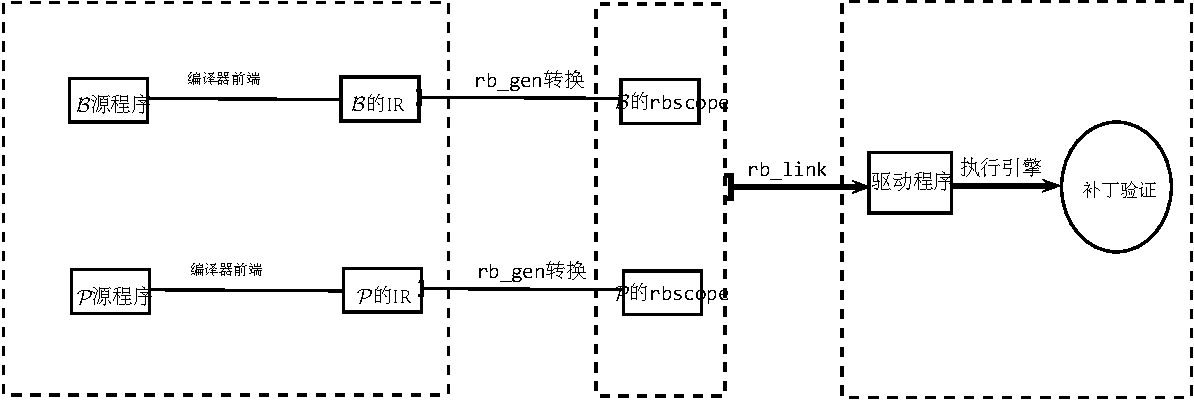
\includegraphics[width=.95\textwidth]{fig/workflow.pdf}\\
    \end{center}
  \end{figure}
  \end{alertblock}}}
\end{frame}

\section{\rbscope 的生成}

\begin{frame}
  \transblindsvertical<2>
  \frametitle{\rbscope 的生成流程}
  \begin{columns}
    \column{.45\textwidth}
    \vspace{-30pt}
    \begin{figure}[t]
      \begin{center}
        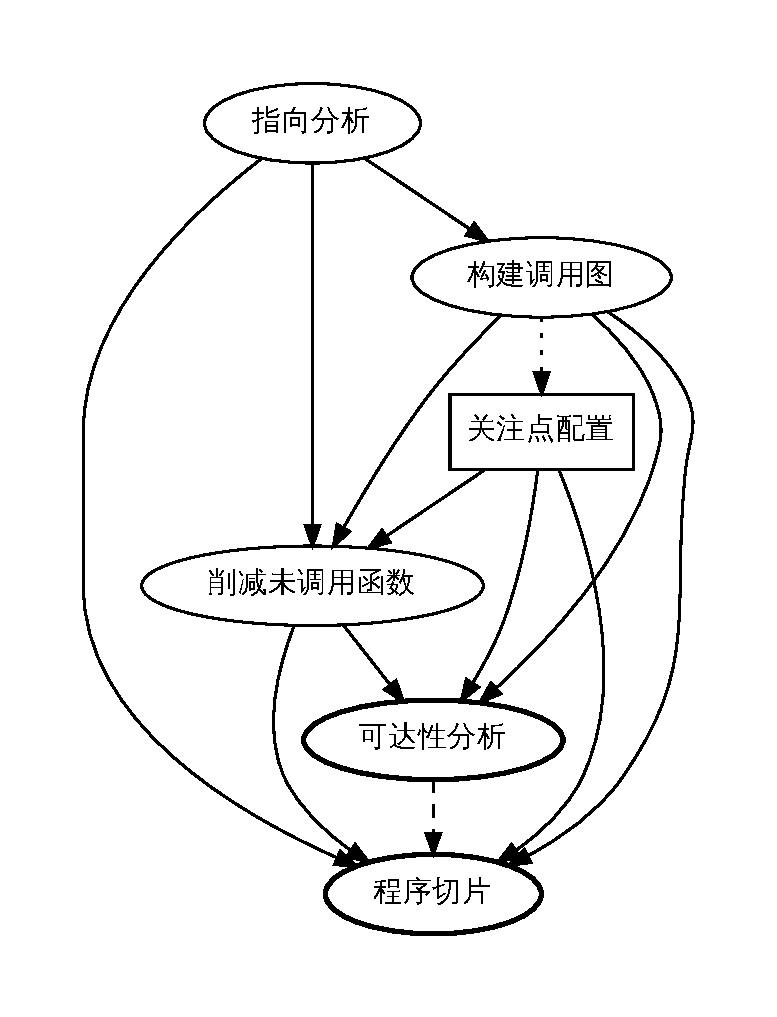
\includegraphics[height=.85\textheight]{fig/rb_gen.pdf}
      \end{center}
    \end{figure}
    \column{.45\textwidth}
    \pause
    \footnotesize{
      通过程序削减生成\rbscope 的过程需遵循下面的基本原则:
      \begin{itemize}
      \item[\ding{223}] 保留下的程序必须包含\structure{所有}可能执行的代码,即削减过程必须是保守的。
      \item[\ding{223}] 保留下的程序在添加了驱动程序之后必须是\structure{可执行}的。
      \item[\ding{223}] 出于选择性符号执行要求,削减程序过程应该尽可能\structure{精确}。
      \end{itemize}
    }
  \end{columns}
\end{frame}

\begin{frame}
  \frametitle{关注点配置}
    \begin{block}{}
  \begin{itemize}
  \item[\ding{224}] 根据C源文件的\emph{配置信息}在LLVM IR层次添加元数据
    \begin{enumerate}
    \item 入口函数\prog\entry : 指定函数名称(\textit{手动}或\textit{自动})
    \item 程序出错位置\prog\bs : 局限于$\_\_assert\_fail$
    \item 程序补丁部分\prog\ps : 粗略精确到到程序基本块层次
    \end{enumerate}
  \item[\ding{224}] 由元数据解析得到中间形式下的关注点信息
  \end{itemize}
    \end{block}
\end{frame}

\begin{frame}[containsverbatim]
  \frametitle{自动确定入口函数的算法}
  \centering{\scalebox{0.75}{%
      \begin{algorithm*}[H]
        \caption{入口函数定位算法}
        \SetAlgoNoLine
        将直接包含 \prog\ps 的函数标记为 $\mathcal{F}{_{pfn}}$, 直接包含 \prog\ps 的函数标记为 $\mathcal{F}{_{pfn}}$

        根据调用图,计算得到所有直接或通过函数指针间接调用 $\mathcal{F}{_{pfn}}$ 的函数集合$\mathcal{F}_{p}$; 计算可以调用$\mathcal{F}_{p}$所有函数的闭包,记为$\widehat{\mathcal{F}_{p}}$

        根据调用图,计算得到所有直接或通过函数指针间接调用 $\mathcal{F}{_{bfn}}$ 的函数集合$\mathcal{F}_{b}$; 计算可以调用$\mathcal{F}_{b}$所有函数的闭包,记为$\widehat{\mathcal{F}_{b}}$

        计算$\widehat{\mathcal{F}_{p}}$ 和$\widehat{\mathcal{F}_{b}}$的共同主调函数,将之作为入口函数\prog\entry
      \end{algorithm*}}}

\end{frame}

\begin{frame}
  \frametitle{调用图的建立}
\centering\doublebox{\scriptsize{LLVM \textit{框架自身提供的调用图过于粗糙,{\alert{准确}}的调用图算法实现如下:}}}\\
\vspace{10pt}
  \centering{\scalebox{0.75}{
\begin{algorithm}[H]
\caption{准确调用图的生成}
\SetAlgoNoLine
遍历整个编译单元,当遇到调用点,转至2

若该调用处的值为函数常量,则将该主调函数和被调函数对加入直接调用的directCaller2CalleeMap中;若该调用点为间接调用,通过指向分析找出该变量所指向的所有可能的值,将主调函数和这些值结对加到directCaller2CalleeMap中。记录被调函数和调用点信息于directCallee2CSMap中。

重复上述两步直至遍历完成。将所有的直接调用的caller到callee的映射(directCaller2CalleeMap)传递给间接调用的caller到callee的映射(Caller2CalleeMap)。
\end{algorithm}
    }}
\end{frame}


\begin{frame}[containsverbatim]
  \frametitle{一个关于调用图的例子}
  \begin{columns}
    \column{.45\textwidth}
\begin{lstlisting}[language={[ANSI]C}]
  int dec(int i) { return i - 1; }
  
  unsigned long func1(int i) {
    if (i == 0) return 1;
    return func1(dec(i)) * i;
  }
  
  unsigned long func2(int i) { 
    return i * 0;
  }
  
  unsigned long (*pF)(int) = func1;
  
  int getNextRandomValue(void) { 
    return rand() % 10; 
  }
  
\end{lstlisting}
  \column{.45\textwidth}
\begin{lstlisting}[language={[ANSI]C}]
  void populate_array(int *array, 
    size_t arraySize, int (*getNextValue)(void)) {
    for (unsigned i = 0; i < arraySize; i++)
     array[i] = getNextValue();
  }

  int main(void) {
    int i = 3;
    int myarray[10];
    if (i < 3) {
      pF = func1;
    } else {
      pF = func2;
    }
    pF(getNextRandomValue());
    populate_array(myarray, 10,  getNextRandomValue);
  }
\end{lstlisting}
\end{columns}  
\end{frame}

\begin{frame}
  \frametitle{不同的调用图}
  \begin{columns}
    \column{.48\textwidth}
  \begin{alertblock}{}
    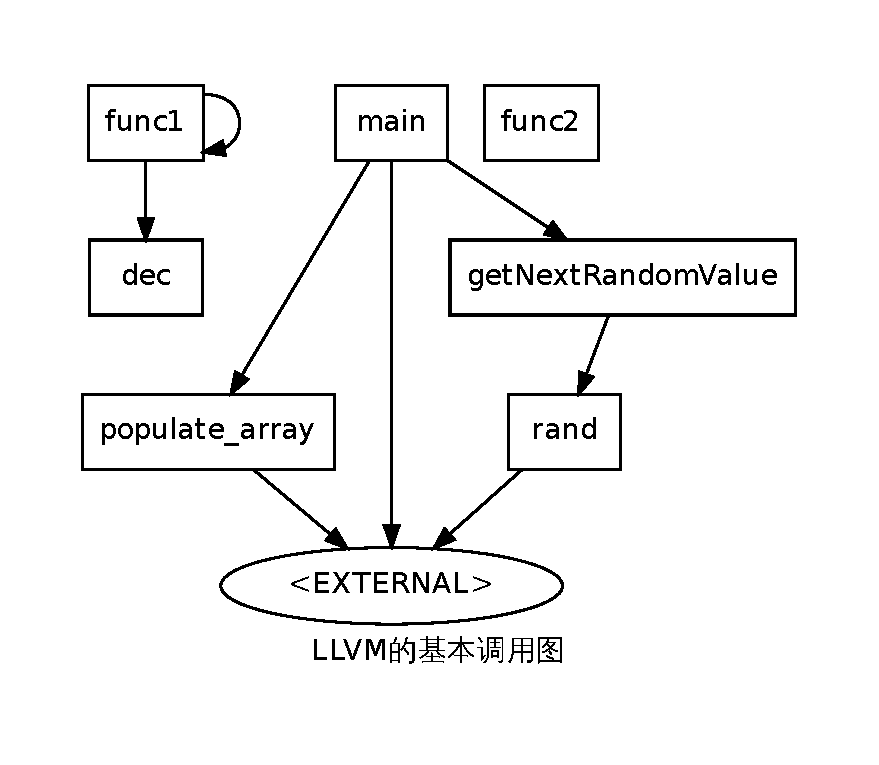
\includegraphics[width=\textwidth, height=.6\textheight]{cg_llvm.pdf}
  \end{alertblock}
    \column{.42\textwidth}
  \begin{alertblock}{}
    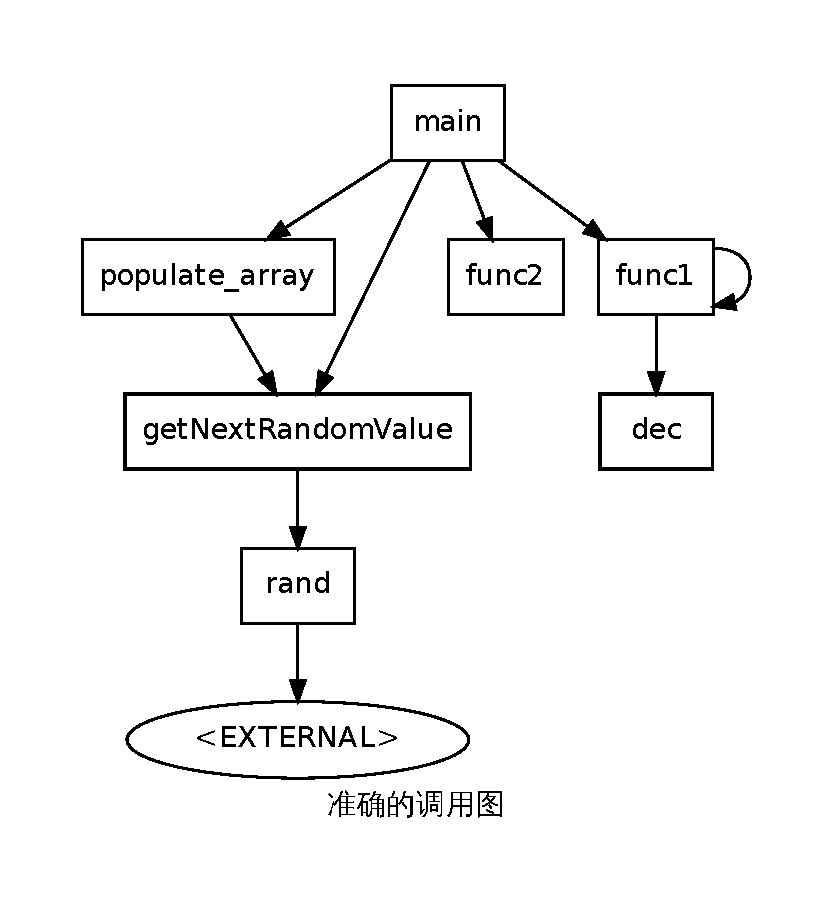
\includegraphics[width=\textwidth, height=.6\textheight]{cg.pdf}
  \end{alertblock}
  \end{columns}
\end{frame}

\begin{frame}
  \frametitle{基于关注点可达性的削减}
  \transboxin<2>
  \vspace{2pt}
  \only<1>{\centering\scalebox{0.75}{
\begin{algorithm}[H]
\caption{可达性算法}
\SetAlgoNoLine

将每个基本块以函数调用点为界限划分为多个“子基本块”。初始认为仅关注点所在子基本块可达。

(1)在过程内计算可达性,更新该子基本块为可达。(2)将可达调用点的所有未完全被访问(函数中至少存在一个调用点未被访问)的被调函数及该被调函数的所有未完全被访问的callee(Caller2CalleeMap)的所有基本块都更新为可达,标记所有的callee的所有调用点为已访问。

根据directCallee2CSMap得到关注点所在函数的所有未被访问的被调用点(采用队列的方式)。
将每个被调用点作为间接关注点,标记重复step2,step3中的操作直至(1)所有函数中的调用点都被访问过。
\end{algorithm}}}

\only<2>{\centering\doublebox{在保证程序语义正确的基础上进行削减}}
\end{frame}

\section{补丁验证}

\begin{frame}
  \frametitle{单程序的补丁验证}
  \centering\scalebox{0.75}{
\begin{algorithm}[H]
\caption{单程序的补丁验证}
\SetAlgoNoLine

将原本属于本编译单元的全局变量通过符号化函数$klee\_make\_symbolic$转化为“符号变量”。

为\prog\entry 中的函数参数在编译单元模块上分配存储空间(类似于全局变量)。根据变量的类型信息,将这些全局变量转化为“符号变量”。

将函数中所关注的\prog\ass 转化为条件分支语句$if\ldots else$的形式,当满足assert被触发的条件时对应的标记位为\textsl{True}。

给编译单元添加main函数(若入口函数本身为main函数则需将之重命名以示区别),将上述转化而来的“符号变量”以实参形式带入函数中。

根据最弱前置条件给符号化的变量通过$klee\_assume$接口添加前置条件。

使用KLEE对新生成的编译单元进行符号执行,从得到的符号执行结果中得到该\rbscope 对应的原有程序的正确性。
\end{algorithm}}
\end{frame}

\begin{frame}[containsverbatim]
  \frametitle{交叉验证的伪代码表示}
  \begin{columns}
    \column{.45\textwidth}
\begin{lstlisting}[language={[ANSI]C}]
   int patch_error = 0, bug_error = 0;
   void cross_validate() {
     if (bug_error && patch_error)
       assert(0, "incomplete patch!");
     else if (bug_error && !patch_error)
       assert(0, "bug fixed!");
     else if (!bug_error && patch_error)
       assert(0, "regression patch!");
     else
       assert(0, "correct and no change!");
   }

   int main(void) {
     make_symbolic(symargs);
     buggyRB();
   }
\end{lstlisting}

    \column{.45\textwidth}
\begin{lstlisting}[language={[ANSI]C}]
  void patchedRB() {
    /* the rbscope of patch program */
    {
      ...
      // replace patch program assert
      patch_error = 1;
    }
    cross_Validate();
  }

  void buggyRB(void) {
    /* the rbscope of buggy program */
    {
      ...
      // replace bug program assert
      bug_error = 1;
      patchedRB();
    }
  }
\end{lstlisting}

  \end{columns}
\end{frame}

\section{\dryrun 的使用}

\begin{frame}
  \frametitle{\secname}
  \begin{itemize}
  \item[\ding{43}] 给定程序\prog ,通过提供的Emacs扩展将\prog\entry , \prog\bs , \prog\ps 信息写入配置文件config.json中。
  \item[\ding{43}] 将\prog 通过llvm-gcc(或clang)转换成LLVM的中间形式
  \item[\ding{43}] 装载LLVM的opt扩展rb\_gen,根据需要执行下面的转换
    \begin{enumerate}
    \item \textmd{rb-md} 将config.json中的信息以元数据形式写入LLVM的IR中
    \item \textmd{rb-uncall} 删除编译单元中未被调用函数
    \item \textmd{rb-reach} 分析对\prog\ps 和\prog\bs 的过程间可达性,并依此削减程序
    \item \textmd{rb-slice} 对得到的程序进行过程间切片
    \end{enumerate}
  \item[\ding{43}] 利用驱动程序合成工具\textmd{rb\_link},添加程序入口及符号执行语义,得到klee-input.bc
  \item[\ding{43}] 调用KLEE对klee-input.bc进行符号执行
  \end{itemize}
\end{frame}

\part{实验与评估}
\frame{\partpage}

\begin{frame}
  \frametitle{测试用例及\rbscope 生成}
  \begin{table}
    \centering
    \tiny
    \begin{tabular}{|c|c|c|c|c|c|c|c|}
      \hline
      编号 & 程序名 & \patch\ps & \patch\bs 行号 & 类型 & \patch\scope 大小(Kb) & $T_{rbc}$(ms)& \patch 大小(Kb) \\
      \hline
      01 & cut & 620 & 624 &  添加 &2.6 & 106 & 181\\ \hline
      02 & factor & 114 & 121 &  修改 & 2.2 & 62 & 139\\ \hline
      03 & join & 642 & 586 & 修改 & 1.8& 54& 168\\ \hline
      04 & mv & 461 & 465 &  修改 & 2.8 & 62 & 404 \\ \hline
      05 & od & 881 & 991 &  修改 & 2.0 & 60 & 193 \\ \hline
      06 & od & 1,290 & 1,389 &  修改 & 3.7 & 60 & 193\\ \hline
      07 & rm & 322 & 347 &  修改 & 1.8 & 71 & 257 \\ \hline
      08 & tail & 139 & 638 &  修改 & 2.7 & 89 & 210 \\ \hline
      09 & tr & 419 & 1,107 & 修改 & 2.1 & 56 & 187 \\ \hline
      10 & tr & 898 & 810 &  修改 & 8.9 & 55 & 187 \\ \hline
      11 & tr & 422 & 1,107 & 删除 & 2.2 & 54 & 187 \\ \hline
      12 & tsort & 140 & 170 &  修改 & 4.9 & 63 & 141 \\ \hline
    \end{tabular}
    \label{tab:cases}
  \end{table}
\end{frame}

\begin{frame}
  \frametitle{对补丁验证的可行性和高效性的评估}
  \vspace{-8pt}
  \begin{table}
    \centering
    \tiny
    \begin{tabular}{|p{0.80cm}|c|c|c|c|r|}
      \hline
      编号 & 版本 & 是否有效 & 验证时间(s)& 指令数(K) & 查询次数 \\
      \hline
      \multirow{2}{0.80cm}{01}
      & $rb\_scope$ &是 &  0.47  & 5.1 & 63  \\  \cline{2-6}
      & original &  否 & 超时 &   84,869.0 & 3,968  \\
      \hline
      \multirow{2}{0.80cm}{02}
      & $rb\_scope$ &否 & 0.49 & 6.2 & 120  \\  \cline{2-6}
      & original & 是 & 57.251 &  137.1 & 504  \\
      \hline
      \multirow{2}{0.80cm}{03}
      & $rb\_scope$ &否 & 1.09 & 9.8 & 69  \\  \cline{2-6}
      & original &  否 & 超时 &  1,433,000.1 & 4,319  \\
      \hline
      \multirow{2}{0.80cm}{04}
      & $rb\_scope$ &是 &  1046.17 & 1,027.4 & 4,121  \\  \cline{2-6}
      & original & 否 & \alert{x} &  \alert{x} & \alert{x}  \\
      \hline
      \multirow{2}{0.80cm}{05}
      & $rb\_scope$ &是 &  26.80 & 6.7 & 338  \\  \cline{2-6}
      & original & 否 & 超时 &  363,301.0 & 1,983   \\
      \hline
      \multirow{2}{0.80cm}{06}
      & $rb\_scope$ &是 &  3.48 & 5.3 & 74  \\  \cline{2-6}
      & original & 否 &超时  & 276,434.2 & 7,0982  \\
      \hline
      \multirow{2}{0.80cm}{07}
      & $rb\_scope$ &是 &  1.02 & 5.5 & 77  \\  \cline{2-6}
      & original & 是 & 1.06 & 18.9   & 148  \\
      \hline
      \multirow{2}{0.80cm}{08}
      & $rb\_scope$ &是 &  1.80 & 5.2 & 60  \\  \cline{2-6}
      & original & 否 & 超时 &  2,422,569.1 & 270  \\
      \hline
      \multirow{2}{0.80cm}{09}
      & $rb\_scope$ &是 &  3.41 & 18.5 & 79  \\  \cline{2-6}
      & original & 否 & 超时 &  245.7 & 775  \\
      \hline
      \multirow{2}{0.80cm}{10}
      & $rb\_scope$ &是 &  2.64 ms & 6.1 & 13  \\  \cline{2-6}
      & original & 是 & 672.69  &  1,299.6 & 3,021  \\
      \hline
      \multirow{2}{0.80cm}{11}
      & $rb\_scope$ &是 &  20.13 & 2.3 & 838  \\  \cline{2-6}
      & original & 否 & 超时  &  4,521.9 & 8,432  \\
      \hline
      \multirow{2}{0.80cm}{12}
      & $rb\_scope$ &是 &  3.02 & 5.5 & 88  \\  \cline{2-6}
      & original & 否 & 超时 &  4,651.3 & 4,648  \\
      \hline
    \end{tabular}
    \label{tab:eval1}
  \end{table}
\end{frame}

\begin{frame}
  \transdissolve<2->
  \frametitle{对回归错误和错误肯定的评估}
  \begin{table}
    \centering
    \tiny
    \begin{tabular}{|l|c|c|c|r|}
      \hline
      编号 & \textit{回归错误} & $T_{cv}$(s) & \textit{错误肯定} &$T_{fp}$(s) \\
      \hline
      01 & 是 & 1.08 & 否 & 0.79 \\ \hline
      02 & - & 超时 & - &超时\\ \hline
      03 & 是 & 1.09 & 否 &5.64\\ \hline
      04 & - & 超时 & - &超时\\ \hline
      05 & - & 超时 & - &超时\\ \hline
      06 & 是 & 114.54 & 否 & 540.84\\ \hline
      07 & \alert<3->{否} & 9.17 & \alert<2->{是} & 2.09\\ \hline
      08 & \alert<3->{否} & 7.26 & 否 & 8.50\\ \hline
      09 & 是 & 2.01 & 否 & 8.03\\ \hline
      10 & - & 超时 & - &超时\\ \hline
      11 & 是 & 2.11 & 否 & 93.40\\ \hline
      12 & 是 & 3.02 & 否 & 7.94\\ \hline
    \end{tabular}
    \label{tab:eval2}
  \end{table}
\end{frame}

\part{总结与展望}
\label{part:summary}
\frame{\partpage}

\begin{frame}
  \transboxin
  \frametitle{总结}
  \begin{center}
  \begin{block}{}
    \begin{itemize}
      \item 展示了一种结合静态分析手段和动态符号执行的程序验证的新方法
      \item 在开源编译器框架LLVM、符号执行引擎KLEE及STP约束求解器的基础上实现了
        反映该思想的工具\dryrun
      \item 从GNU Coreutils程序集合选取了数十个补丁程序分别针对\dryrun 的\textit{高效性}、
        \textit{有效性}、\textit{回归错误}及\textit{程序错误肯定}等方面进行评估,实验的结果说明通过剔除不相关代码
        而有选择地进行符号执行的思路是可行的
    \end{itemize}
  \end{block}
  \end{center}
\end{frame}

\begin{frame}
  \transblindshorizontal
  \frametitle{缺陷与不足}
  \begin{itemize}
\item[\ding{235}] \dryrun 并没有对符号执行工具KLEE的核心算法做修改,因此它受限于KLEE的执行机制
\item[\ding{235}] 尽管通过程序削减减少了程序的大小,然而保留下来的程序中仍然可能存在大量的分支循环结构,这种情况下符号执行的代价仍然很大
\item[\ding{235}] 忽略了程序实际执行时的该参数的前置条件,增大了符号执行的开销
  \end{itemize}
\end{frame}

\begin{frame}
  \transboxout
  \frametitle{未来的改进}
  \begin{block}{}
      \begin{itemize}
  \item[\ding{37}] 结合LLVM提供的编译优化,优化Andersen指向分析算法在LLVM IR上的
    实现
  \item[\ding{37}] 在程序依赖图上采用更精确的过程间切片
  \item[\ding{37}] 通过静态分析的方法得到程序执行到\rbscope 时的最弱前置条件给出符号变量的上下界
  \item[\ding{37}] 不直接削减程序本身而采用添加注解(annotation)的方式标记程序中的\rbscope ,并以此修改KLEE执行方式
  \item[\ding{37}] 使用\textbf{$S^2E$}等扩展性更好的符号执行框架
  \end{itemize}

  \end{block}
\end{frame}

\appendix
\begin{frame}
  \transdissolve
  \begin{centering}
    \Huge\color{green!60!black} {\shuti{谢谢各位老师!}}\par
  \end{centering}
\end{frame}

\end{document}